\documentclass[11pt]{article}

\usepackage[utf8]{inputenc}  %francais et caractères
\usepackage[T1]{fontenc} 
\usepackage[francais]{babel}

\usepackage{amsmath} %math
\usepackage{amssymb}

\usepackage{graphicx} %images
%\usepackage{caption}
\usepackage{subfig}
%\usepackage{subcaption}
\usepackage{wrapfig} %images dans texte

\usepackage[table,xcdraw,dvipsnames]{xcolor} %couleurs
\usepackage{appendix} %annexes
\usepackage{listings} %insertion de lignes de code
\usepackage{physics}
\usepackage{mathtools, stmaryrd}
%\usepackage[framed,numbered,autolinebreaks,useliterate]{mcode}

\usepackage[right=2cm, left=2cm, top=2cm, bottom=2cm, headheight=110pt]{geometry}
\usepackage{lscape}

\usepackage{fancyhdr}
\pagestyle{fancy}
\fancyhf{}
\fancyhead[R]{\leftmark}
\fancyhead[L]{PR 214}
\cfoot{\thepage}

\usepackage[nottoc]{tocbibind} % Rajoute la bibliographie dans la tdm

%Tables du generateur de tables
\usepackage[normalem]{ulem}
\useunder{\uline}{\ul}{}

\renewcommand\lstlistingname{Code}
\renewcommand{\lstlistlistingname}{Table de Codes}

\lstset{language = C,%
    %basicstyle=\color{red},
    breaklines=true,%{}
    keywordstyle=\color{Orange},
    identifierstyle=\color{Cyan},
    stringstyle=\color{Red},
    commentstyle=\color{Green},
    morekeywords={matlab2tikz},
    morekeywords=[2]{1}, keywordstyle=[2]{\color{black}},
    showstringspaces=false,%without this there will be a symbol in the places where there is a space
    numbers=left,%
    numberstyle={\tiny \color{black}},% size of the numbers
    numbersep=9pt, % this defines how far the numbers are from the text
    emph=[1]{for,end,break},emphstyle=[1]\color{red}, %some words to emphasise
    %emph=[2]{word1,word2}, emphstyle=[2]{style}, 
    backgroundcolor=\color{White},
    basicstyle=\scriptsize\color{black}\ttfamily,
    frame=L,
    captionpos = b,
    %===========================================================
    framesep=3pt,%expand outward.
    framerule=0.4pt,%expand outward.
    xleftmargin=3.4pt,%make the frame fits in the text area. 
    xrightmargin=3.4pt,%make the frame fits in the text area.
    %=========================================================== 
    rulecolor=\color{Red}   
}


\newcommand{\HRule}{\rule{\linewidth}{0.5mm}}

\newenvironment{rmq}[1] {\noindent\HRule\par\vspace{5pt}\textbf{\textit{REMARQUE : }}#1}{\\\HRule\par\vspace{5pt}}



\begin{document}

% Page de Garde
\thispagestyle{empty}

\noindent 
DURAND Clovis \\ MARINO Xavier\hfill{4 Mai 2017}
% // et entrer d'autres noms. 



\vspace{2cm}
\begin{center}
\Large{PR 214} % Inserer la matiere concernée
\HRule \\[0.1cm]
{\textsc{\LARGE \textbf{Projet Thématique\\ Conception d'un module en VHDL pour la gestion d'un Pmod OLEDrgb Digilent sur FPGA}}}\\
\HRule\\[01cm]
\Large{V1.0} % Version of document
\end{center}
\vspace{1,5cm}

\begin{figure}[htbp]
\begin{center}
\includegraphics[width=10cm]{/Users/Clovel/Documents/Scolaire/ENSEIRB-MATMECA/Logo_ENSEIRB.png}
\end{center}
\end{figure}

\vspace{1cm}
\begin{center}
\Large{ENSEIRB-Matmeca \\ Bordeaux - Talence}
\end{center}

\vspace{1cm}
Encadrant : Yannick Bornat

\newpage
% Tables
\tableofcontents
%\lstlistoflistings
\listoffigures
\newpage 

% Debut doc
\setcounter{section}{-1}

\section{Introduction}

Au cours de ce projet, un objectif clair nous a été fixé : afficher une image sur un écran OLED couleur d'une résolution 96 x 64, connecté sur une carte Nexys4 de Digilent. Cet écran est monté sur un Pmod (extensions de cartes d'interfaces Entrées/Sorties de chez Digilent). Le cœur du projet est de comprendre comment le Pmod communique avec la carte Nexys4 et de lui envoyer les informations nécessaires à son fonctionnement, telle que la séquence de commandes initialisation de l'écran ou les données de l'image que l'on souhaite afficher. \\

\subsection{Segmentation et déroulement du projet}

Le projet a donc été séparé en plusieurs parties. 

D'abord, l'étude du composant et de sa datasheet. En effet, le Pmod de Digilent possède sa propre datasheet, mais sur celui-ci est monté un contrôleur spécifique à l'écran OLED : le SSD1331. Il a donc été nécessaire d’appréhender comment celui-ci fonctionnait. 

Ensuite, nous avons élaboré un programme d'initialisation et d'utilisation de l'écran. Un microprocesseur basique à été implémenté sur FPGA, nous compilions des programmes écrit en langage C, et nous testions le Pmod de cette façon. Ainsi, en se basant sur ce qu'on a appris des datasheet, nous avons mis au point une séquence de commandes pour initialiser l'écran et pour lui envoyer, via la liaison UART de la carte Nexys4 les données bitmap de l'image. Le but de ces programmes est avant tout de comprendre ce qui doit être décrit en VHDL pour le module de gestion de notre écran OLEDrgb, et ils ne constituent pas notre produit fini. 

Enfin, nous avons développé notre module de gestion du Pmod en VHDL. L’environnement de travail choisi est Vivado de Xilinx. En appliquant une ingénierie inverse aux programmes C développés en amont, une architecture précise à été définie, et la conception de tous les blocs composant notre module ont été écrits. \\

En pratique, l'étude de la datasheet à été un travail permanent, et à donc été faite en parallèle au développement de nos programmes C et de nos descriptions VHDL. Les points de fonctionnement de nos composant qui semblent pour certains relativement simples en apparence mais nous ont posé problème tout de même quand nous avancions dans nos études. A chaque problème de la sorte, il a fallu revoir les points concernés de la datasheet à plusieurs reprises. Pour les problèmes plus complexes, comme la gestion de la communication entre la carte et le Pmod, la datasheet à été d'une grande aide. 

\clearpage

\section{Pmod OLEDrgb}

Un Pmod est un périphérique ou extension destinée à être utilisé avec des cartes programmables telles que la Nexys4 de Digilent que nous utilisons dans ce projet. Le Pmod sur lequel notre travail se concentre ici est l'OLEDrgb, un écran OLED (Organic Light-Emitting Diode) \cite{oleddef} d'une résolution de 96 x 64 pixels capable d'afficher 65k couleurs. 

\begin{figure}[!htbp]
	\begin{center}
		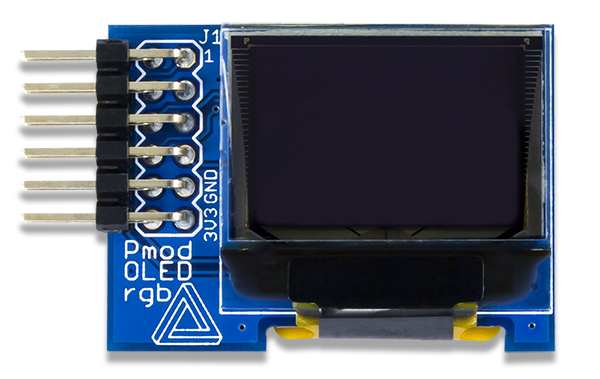
\includegraphics[width = 7cm]{/Users/Clovel/Documents/Scolaire/ENSEIRB-MATMECA/E2/PR214_OLED_project/rapport_PR214_OLEDrgb/pmodoledrgb-1.png}
		\caption[OLEDrgb Pmod]{Le Pmod OLEDrgb de Digilent utilisé dans ce projet}
	\end{center}
\end{figure}

Pour communiquer avec la carte mère, ce périphérique utilise le protocole SPI (Serial Periphéral Interface Bus). Avec ce protocole, on peut envoyer par paquet les informations et commandes nécessaires au fonctionnement de notre écran OLED. 
Un contrôleur Solomon Systech SSD1331 \cite{ssd1331} est employé pour communiquer entre le Pmod support et le composant de l'écran. Grâce à celui-ci, les commandes envoyées sont exploités et traités. De plus, lorsque que ce contrôleur reçoit des informations, il les stocke dans la RAM de l'écran. Ce contrôleur possède tout un panel de commandes qui permettent d'interagir avec l'écran. (i.e. dessiner un rectangle, un pixel, etc.)\\


Ce Pmod à 12 broches : \\
% Generated w/ http://www.tablesgenerator.com/
% Please add the following required packages to your document preamble:
% \usepackage{graphicx}
% \usepackage[table,xcdraw]{xcolor}
% If you use beamer only pass "xcolor=table" option, i.e. \documentclass[xcolor=table]{beamer}
% \usepackage[normalem]{ulem}
% \useunder{\uline}{\ul}{}
\begin{table}[!htbp]
\centering
\resizebox{\textwidth}{!}{%
\begin{tabular}{|c|c|c|c|c|c|c|}
\hline
\multicolumn{7}{|c|}{{\ul \textbf{Header J1}}}                                                                   \\ \hline
Pin & Signal      & Decription             & \cellcolor[HTML]{9B9B9B} & Pin & Signal & Description               \\ \cline{1-3} \cline{5-7} 
1   & CS          & Chip Select            & \cellcolor[HTML]{9B9B9B} & 7   & D/C    & Data/Command Control      \\ \cline{1-3} \cline{5-7} 
2   & MOSI        & Master Out - Slave In  & \cellcolor[HTML]{9B9B9B} & 8   & RES    & Power Reset               \\ \cline{1-3} \cline{5-7} 
3   & \textit{NC} & \textit{Not Connected} & \cellcolor[HTML]{9B9B9B} & 9   & VCCEN  & Vcc Enable                \\ \cline{1-3} \cline{5-7} 
4   & SCK         & Serial Clock           & \cellcolor[HTML]{9B9B9B} & 10  & PMODEN & Vdd Logic Voltage Control \\ \cline{1-3} \cline{5-7} 
5   & GND         & Power Supply Ground    & \cellcolor[HTML]{9B9B9B} & 11  & GND    & Power Supply Ground       \\ \cline{1-3} \cline{5-7} 
6   & VCC         & Power Supply (3.3V)    & \cellcolor[HTML]{9B9B9B} & 12  & VCC    & Power Supply (3.3V)       \\ \hline
\end{tabular}%
}
\caption{My caption}
\label{my-label}
\end{table}

\clearpage





%Bibliographic references
\clearpage
\begin{thebibliography}{9}
\bibitem{oleddef} 
OLED Wikipedia page for definitions\\
https://en.wikipedia.org/wiki/OLED

\bibitem{oledrgb} 
OLEDrgb Pmod reference sheet and Datasheet\\
\textit{Pmod OLEDrgb Reference Manual.} \\
Digilent, Revised April 26, 2016

\bibitem{spidef} 
Definition of Serial Peripherals Interface Bus and how it works\\
https://web.archive.org/web/20150413003534/http://www.ee.nmt.edu/\~teare/ee308l/datasheets/S12SPIV3.pdf\\
Motorola, Inc. , Original Release Date: January 21, 2000, Revised: February 04, 2003

\bibitem{ssd1331}
Datasheet du SSD1331, contrôleur de matrice de points OLED/PLED\\
https://www.parallax.com/sites/default/files/downloads/28087-SSD1331\_1.2.pdf
\end{thebibliography}


















\end{document}